\documentclass[main.tex]{subfiles}
\begin{document}
PPLBench is a benchmark for analyzing and comparing the accuracy and performance of Probabilistic Programming Languages and Libraries (PPLs) over various probabilistic models. It is designed to be open and modular such that contributors can add new models, PPL implementations, and evaluation metrics to the benchmark.

\begin{figure}[h]
  \centering
  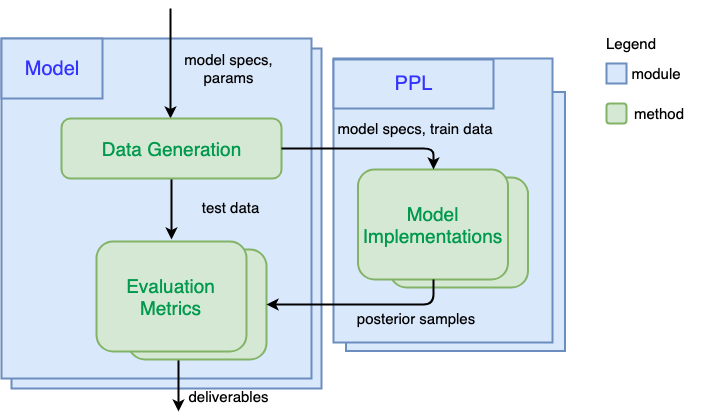
\includegraphics[width=150mm]{figures/system_overview.png}
  \caption{PPLBench system overview}
  \label{fig:fig1}

\end{figure}
PPLBench is implemented in Python 3\cite{Python}.
Each model in PPLBench as well as a model's PPL implementation is a module as seen in figure \ref{fig:fig1}. The typical PPLBench flow is as follows:
\begin{itemize}
\item \textbf{Model Instantiation and Data Generation}: We establish a model $P_\theta(X,Z)$ with ground-truth parameter distributions($\theta \sim P_\phi$) where $\phi$ is the hyperprior.
In some models theta is sampled while in others it can be specified by users. \newline
The model factorizes as:
$$
P_\theta(X,Z) = P_\theta(Z)P_\theta(X|Z)
$$
And sample parameters:
$$
Z_1 \sim P_\theta(Z)
$$
We then simulate train and test data from this model:
$$
X_{train} \stackrel{iid}{\sim} P_\theta(X|Z=Z_1)
$$
$$
X_{test} \stackrel{iid}{\sim} P_\theta(X|Z=Z_1)
$$
Note that this process of data generation is performed independent of any PPL.
\item \textbf{PPL Implementation and Posterior Sampling}: Using the training data, we train various PPL implementations which learn a model $P_\theta(X = X_1,Z)$; obtain $n$ posterior samples of parameters along with runtime information.
$$
Z^*_{1...n} \sim P_\theta(Z | X = X_{train})
$$
PPLBench is designed to accept an approximate time per PPL per iteration.
The PPLBench estimates the number of posterior samples to obtain from the implementations based on this time constraint.
The PPL’s default warmup/burn-in and initialization parameters were left unchanged.
The sampling is restricted to a single chain and any form of multi-threading is disabled.
\item \textbf{Evaluation}: Using the test data $X_{test}$, posterior samples $Z^*_{1...n}$ and timing information, the PPL implementations are evaluated on various evaluation metrics.
The default evaluation metric is average log predictive vs. time for each implemented PPL.
A running average of the log posterior predictive is computed w.r.t $n$ and a further mapping $n$ to the elapsed time is computed.
The final plot is hence a running average posterior predictive w.r.t time.
This metric has been previously used by \cite{kucukelbir2017automatic} to compare convergence of different implementations of statistical models.
$$
Average Posterior Predictive(n) = \frac{1}{n}\sum_{i=1}^{n}\log(P(X_{test}|Z=Z^*_{i}))
$$
After computing the average posterior predictive w.r.t time over each iteration, the min, max and mean values over iterations is obtained.
These are plotted on a graph for each PPL implementation so their convergence behavior can be visualized.
The time axis in the plot is on a log scale to help accommodate larger timescales and vastly different convergence behaviors.
This plot is designed to capture both the relative performance and accuracy of these implementations.
\end{itemize}
Using the PPLBench framework, we establish three models to evaluate performance of PPLs:
\begin{enumerate}
\item Robust regression model with Student-T errors\cite{gelman2013bayesian}
\item Latent Keyphrase Index(LAKI) model, a Noisy-Or Topic Model\cite{liu2016representing}
\item Crowdsourced annotation model, estimating true label of an item given a set of labels assigned by imperfect labelers\cite{passonneau2014benefits}
\end{enumerate}
These models are chosen to cover a wide area of use cases for probabilisic modelling.
All the above models have been implemeted in JAGS\cite{plummer2003jags} and Stan\cite{carpenter2017stan} PPLs.
The model and PPL implementation portfolio is expected to be expanded with additional open-source contributions.
Subsequent sections describe these models and implementations in detail along with analysis of observed results.











































































\end{document}
